\documentclass[dvipdfmx]{jsarticle}
\usepackage[dvipdfmx]{graphicx}
\usepackage{amsmath} % alignに必要
\usepackage{tikz} % 画像
\usepackage{amssymb} % \mathbb に必要
\usetikzlibrary{calc} % TikZに計算させる
\begin{document}

\newcommand{\highlight}[3][yellow]{\tikz[baseline=(x.base)]{\node[rectangle,rounded corners,fill=#1!10](x){#2} node[below of=x, color=#1]{#3};}}

\section{証明 recipe}

\subsection{2項定理}

\subsubsection{命題}
\[ (a + b)^n = \sum_{r=0}^{n} \binom nr a^{n-r}b^r \]

\subsubsection{具体例}
n = 3のとき

\begin{align*}
  (a + b)^3 &= \binom {3}{0} a^{3-0}b^0 + \binom {3}{1} a^{3-1}b^1 + \binom {3}{2} a^{3-2}b^2 + \binom {3}{3} a^{3-3}b^3 \\
            &= a^3 + 3a^2b + 3ab^2 + b^3
\end{align*}

\subsubsection{数学的帰納法による証明}

$自然数nに関する命題S(n)$ を以下のように定める。

\[ (a + b)^n = \sum_{r=0}^{n} \binom nr a^{n-r}b^{r} \]

$n = 1のときS(n)$ は成り立つ。

\begin{align*}
  (a + b)^1 &= \sum_{r=0}^{1} \binom{1}{r} a^{1-r}b^r \\
            &= \binom{1}{0}a^{1-0}b^0 + \binom {1}{1} a^{1-1}b^1 \\
            &= a + b
\end{align*}

出発点はOKなので、次はドミノがずっと倒れることを保証するために、$S(k) \rightarrow (k+1)$ が成り立つか見てみる。つまり

\[ \biggl[ (a + b) ^k = \sum_{r=0}^{k} \binom{k}{r} a^{k-r}b^r \biggl] \rightarrow \biggl[(a + b)^{(k+1)} = \sum_{r=0}^{(k+1)} \binom{(k+1)}{r} a^{(k+1)-r}b^r \biggl] \]

を示せばよい。前提からはじめると

\begin{align*}
(a + b)^k &= \sum_{r=0}^{k} \binom kr a^{k-r}b^r \qquad &\text{(S(k)は前提なので真)} \\
(a + b)^{k+1} &= (a+b) \sum_{r=0}^{k} \binom kr a^{k-r}b^r \qquad &\text{(両辺に(a+b)をかける)} \\
&= a\sum_{r=0}^{k} \binom kr a^{k-r}b^r + b\sum_{r=0}^{k} \binom kr a^{k-r}b^r \qquad &\text{(分配する)} \\
&= \highlight[red]{$\displaystyle a^{k+1}  a\sum_{r=1}^{k}$}{} \binom kr a^{k-r}b^r + b\sum_{r=0}^{k} \binom kr a^{k-r}b^r \qquad &\text{(indexをr=1にする)} \\
&= a^{k+1}  a\sum_{r=1}^{k} \binom kr a^{k-r}b^r + \highlight[red]{$\displaystyle b^{k+1} b\sum_{r=0}^{k-1}$}{} \binom kr a^{k-r}b^r \qquad &\text{(indexの上限をk-1にする)} \\
&= a^{k+1} \sum_{r=1}^{k} \binom kr a^{k+1-r}b^r + b^{k+1} + \sum_{r=0}^{k-1} \binom kr a^{k-r}b^{r+1} \qquad &\text{(シグマの係数を中にいれる)} \\
&= a^{k+1} \sum_{r=1}^{k} \binom kr a^{k+1-r}b^r + b^{k+1} + \sum_{r=0+1}^{k-1+1} \binom {k}{(r-1)} a^{k-(r-1)}b^{(r-1)+1} \qquad &\text{(b側のシグマのindexを調整する)} \\
&= a^{k+1} \sum_{r=1}^{k} \binom kr a^{k+1-r}b^r + b^{k+1} + \sum_{r=1}^{k} \binom {k}{r-1} a^{k+1-r}b^{r} \qquad &\text{(シグマでくくれる)} \\
&= a^{k+1} + b^{k+1} + \sum_{r=1}^{k} \Biggl[ \binom kr a^{k+1-r}b^r + \binom {k}{r-1} a^{k+1-r}b^r \Biggl] \\
&= a^{k+1} + b^{k+1} + \sum_{r=1}^{k} \Biggl[ a^{k+1-r}b^r \Biggl( \binom kr + \binom {k}{r-1} \Biggl)\Biggl] \qquad &\text{($a^{k+1-r}b^r$でくくる)} \\
&= a^{k+1} + b^{k+1} + \sum_{r=1}^{k} \Biggl[ a^{k+1-r}b^r \binom {k+1}{r} \Biggl] \qquad &\text{(パスカルの三角形の定理)} \\
&= a^{k+1} + b^{k+1} + \highlight[red]{$\displaystyle (-a^{k+1})+  \sum_{r=0}^{k}$}{} \Biggl[ a^{k+1-r}b^r \binom {k+1}{r} \Biggl] \qquad &\text{(r=0)} \\
&= a^{k+1} + b^{k+1} -a^{k+1} + \highlight[red]{$\displaystyle (-b^{k+1}) + \sum_{r=0}^{k+1}$}{} \Biggl[ a^{k+1-r}b^r \binom {k+1}{r} \Biggl] \qquad &\text{(k+1)} \\
(a + b)^{(k+1)} &= \sum_{r=0}^{(k+1)} \binom {(k+1)}{r} a^{(k+1)-r}b^r \qquad &\text{(結論にたどり着いた!)}
\end{align*}


\section{Algorithm}

\subsection{$\mathcal{O}$ notation}

与えられた関数$g(n)$に対して、$\mathcal{O}(g(n))$によって関数の集合


\[ \mathcal{O}(g(n)) = \{ f(n): ある正の定数c, n_0が存在して、すべてのn \ge n_0に対して0 \le f(n) \le cg(n)を満たす\} \]


を表現する。

入力が一定数以下はオーバーヘッドがあったりで、ノイズなので入力が一定数以上を表現するために$n_0$を設けている。

\section{$\sum$}

\subsection{操作}

\subsubsection{定数倍}
\[ \sum_{k=1}^{n}ma_k = m\sum_{k=1}^{n}a_k \]

定数はくくり出せる。n = 3とすると
\[ \sum_{k=1}^{3}ma_k = (ma_1 + ma_2 + ma_3) = m(a_1 + a_2 + a_3) = m\sum_{k=1}^{3}a_k \]

\subsubsection{分配}

\[ \sum_{k=1}^{n}(a_k + b_k) = \sum_{k=1}^{n}a_k + \sum_{k=1}^{n}b_k  \]

分配法則が成り立つ。 n = 3とすると
\[ \sum_{k=1}^{3}(a_k + b_k) = (a_1 + b_1) + (a_2 + b_2) + (a_3 + b_3) = (a_1 + a_2 + a_3) + (b_1 + b_2 + b_3) = \sum_{k=1}^{3}a_k + \sum_{k=1}^{3}b_k \]

\subsubsection{和の範囲を変える}

\[ \sum_{k=1}^{n}a_k = a_1 + \sum_{k=2}^{n}a_k \]

数列のSumをとっているので、範囲を変えられる。最初の項をはずしたり、最後の項をはずしたり。 n = 3とすると
\[ \sum_{k=1}^{3}a_k = (a_1 + a_2 + a_3) = a_1 + (a_2 + a_3) = a_1 + \sum_{k=2}^{3}a_k \]

\subsubsection{indexを調整する}

\[ \sum_{k=0}^{n}a_k = \sum_{k=0+(i)}^{n+(i)}a_{k-(i)} \]

indexを変更しても、項に渡す前に調整すれば、結果的に生成される数列はかわらない
\[ \sum_{k=0}^{n}2^{k+1} = \sum_{k=1}^{n+1}2^k \]

\section{整数}

\subsection{素数}

\subsubsection{定義}

1以外の自然数で1と自身以外に正の約数をもたない数を素数(prime number)という。

1でも素数でもない数を合成数(composite number)という。

\subsubsection{素数の判定}

$素数 \lor 合成数$ が成り立つので、合成するを判定することで素数の判定もできる。合成数の判定に合成数の以下の性質を利用する。

\[Nが合成数 ならば 1 < a < \sqrt{N} を満たす約数aを1つ以上もつ\]

\[1 < a < \sqrt{N}を満たす約数aが一つも存在しない ならば Nは合成数でない(対偶) \]

この性質から、ある整数Nにおいて、$[2, \sqrt{N}]$の範囲に約数がなければ、$Nは合成数でない \equiv 素数$ が成り立つ。以下証明

Nは合成数なので、定義から1以外の2つの積に分解できる。小さいほうをaとすると

\begin{align*}
  N &= a \times b \qquad ( 1 < a \leq b, \ \ a, b \in\mathbb{Z}) \\
  N &= a \times b \geq a \times a = a^2 \qquad \text{($1 < a \leq b $)} \\
  N &\geq a^2 \\
  a &\leq \sqrt{N}
\end{align*}

この事実を証明したので、心置きなく、素数判定のfor loopに対象判定Nの平方根を終了条件にできる。

\subsection{ユークリッド互除法}

\subsubsection{証明}

2つの整数a,bが与えられたとき、a,bの最大公約数が知りたい.a,bを以下のように表現したとき、aとbの公約数の集合はaとrの公約数の集合と等しくなる。

\[ b = qa + r \ (0 <= r < a)\]

$d | a \land d | b \equiv d | a \land d | r $を証明する。

戦略として、 $(d | a \land d | b \rightarrow d | a \land d | r) \land (d | a \land d | r \rightarrow  d | a \land d | b) $を証明する。
\\\\
(1) $d | a \land d | b \rightarrow d | a \land d | r$ の証明 \\
仮定より、$\exists q_a, q_b ( a = q_ad, b = q_bd)$

\begin{align*}
  b &= aq + r \\
  q_bd &= (q_ad)q + r \qquad \text{(仮定からaとbを置換)} \\
  r &= q_bd - qq_ad \\
  r &= d(q_b - qq_a)
\end{align*}
ここで、 $q_b, q_a, q$ は整数であり、整数の掛け算、引き算は整数に閉じるので$(q_b - qq_a)$は整数。
  したがって、$\exists n ( r = dn) がいえるので、 d | r$がいえる。よって、
  $d | a \land d | b \rightarrow d | a \land d | r$
\\\\
(2) $d | a \land d | r \rightarrow d | a \land d | b$ の証明 \\
仮定より、$\exists q_a, q_r ( a = q_ad, r = q_rd)$

\begin{align*}
  b &= aq + r \\
  b &= (q_ad) + q_rd \qquad \text{(仮定からaとrを置換)} \\
  b &= d(q_a + q_r)
\end{align*}

(1)と同様に、$q_a, q_r$は整数であり、整数に閉じるので、$(q_a + q_r)$は整数。したがって、 $\exists n ( b = dn)$がいえるので、 $d | b$が成り立つ。よって、 $d | a \land d | r \rightarrow d | a \land d | b$ がいえる。

\subsubsection{帰結}
ある2つの数a,bが与えられた時、aとbの約数はaとrの約数でもある。そしてrはbをaで割ったときの余りなのでaよりも小さい。そのため、問題をより小さい問題に言い換えることができる。またaとrの約数は、$a = d_1r + r_2$ とした場合 $rとr_2$の約数でもある。この操作を繰り返すと、diviser(最初のa)がtarget(最初のb)を割り切る(r=0)ときがきて、そのとき、diviserと0(r)がtargetとdiviserの約数となる。そしてそのときのdiviserを最大公約数と呼ぶ(定義)

\subsection{倍数の判定}

3桁の数Nは 100a + 10b + c とあらわせる。

$ N = 2(50a + 5b) + c$ とあらわせるので、Nが2の倍数になるかどうかは最後の桁が2の倍数かどうかによる。

$ N = 100a + 10b + c = 99a + a + 9b + b + c = 3(33a + 3b) + a + b + c$ なので、各桁の数の合計が3の倍数になるかでNが3の倍数かどうか判定できる

\section{統計}

\subsection{組み合わせの数}

\[ \binom nr = \frac{n!}{r!(n-r)!} \]


\subsubsection{組み合わせの漸化式}

\[ \binom nr + \binom {n}{r+1} = \binom {n+1}{r+1} \]

これは、$n+1 = n', r+1 = r' とおくと,  n = n' -1, r = r' -1$と表せるので,以下のようにもかける。

\[ \binom {n'-1}{r'-1} + \binom {n'-1}{r'} = \binom {n'}{r'} \]

\subsubsection{組み合わせの漸化式の証明}

\begin{align*}
&\binom nr + \binom {n}{r+1} \\
&= \frac{n!}{r!(n-r)!} + \frac{n!}{(r+1)!(n-(r+1))!} \qquad &\text{(組み合わせの定義から)} \\
&= \highlight[red]{$\displaystyle \frac{r+1}{r+1} $}{} \cdot \frac{n!}{r!(n-r)!} + \highlight[red]{$\displaystyle \frac{n-r}{n-r} $}{} \cdot \frac{n!}{(r+1)!(n-(r+1))!} \qquad &\text{(通分の準備)} \\
&= \frac{(r+1) \cdot n!}{(r+1)!(n-r)!} + \frac{(n-r) \cdot n!}{(r+1)!(n-r)!} \qquad &\text{(分母を計算)} \\
&= \frac{(r+1) \cdot n! + (n-r) \cdot n!}{(r+1)!(n-r)!} \\
&= \frac{((r+1)+(n-r))n!}{(r+1)!(n-r)!} \qquad &\text{(n!でくくる)} \\
&= \frac{(n+1) \cdot n!}{(r+1)!(n-r)} \\
&= \frac{(n+1)!}{(r+1)!(n-r)!} \\
&= \binom {n+1}{r+1}
\end{align*}

\subsubsection{組み合わせの漸化式の意味}

これは、4枚のカードA,B,C,Dから2枚の組み合わせは、Aを選ばない場合とAを選ぶ場合にわけて考えることができるということを主張している。Aを選ばない場合は、B,C,Dの3つから2つ選ぶことになり、$\binom {3}{2}$, Aを選ぶ場合は、B,C,Dから残りの1つを選ぶことになるので$\binom {3}{1}$. 2つの場合を足すと、$\binom {4}{2}$の組み合わせになるということ。

\subsection{条件つき確率}

2つの事象A,Bに対し、Aが起こった状況のもとでBが起こる条件つき確率といい、以下のように表す

\[ P(B|A) = \frac{P(A \cap B) }{P(A)} \]

考え方としては、$P(B|A)$をgivenとして与えられている事象Aの個数と事象AかつBの個数と捉えて以下のように導く

\begin{align*}
  P(B|A) &= \frac{n(A\cap B)}{n(A)} \\
         &= \frac{\frac{n(A\cap B)}{n(U)}}{\frac{n(A)}{n(U)}} \qquad \text{(分子,分母をn(U)で割る)} \\
         &= \frac{P(A \cap B)}{P(A)}
\end{align*}

条件付き確率を以下の形にしたものを乗法定理という。

\[ P(A \cap B) = P(B|A) \cdot P(A) \]

\subsection{ベイズの定理}

\begin{align*}
  P(X \cap Y) &= \frac{n(X \cap Y)}{n(U)} \\
  &= \frac{n(X \cap Y)}{1} \cdot \frac{1}{n(U)} \\
  &= \frac{n(X \cap Y)}{n(X)} \cdot \frac{n(X)}{n(U)} \\
  &= P(Y|X) \cdot P(X) \\
  \text{同様に} \\
  P(X \cap Y) &= \frac{n(X \cap Y)}{n(U)} \\
  &= \frac{n(X \cap Y)}{1} \cdot \frac{1}{n(U)} \\
  &= \frac{n(X \cap Y)}{n(Y)} \cdot \frac{n(Y)}{n(U)} \\
  &= P(X|Y) \cdot P(Y) \\
  \text{従って} \\
  P(Y|X)P(X) &= P(X|Y)P(Y) \\
  \highlight[red]{$\displaystyle P(X|Y)$}{事後確率} &=
    \highlight[red]{$\displaystyle P(X)$}{事前確率}
    \cdot
    \highlight[blue]{$\displaystyle \frac{P(Y|X)}{P(Y)}$}{修正項}
\end{align*}

\section{Burn Mathclass}

\subsection{分数}
$\frac{1}{n}$ はnをかけると1になる数として定義する。これでうっかり騙されて割り算というものを使わされることを防げる。だから、$\frac{15}{72}は(15)(\frac{1}{72})$の略号でしかない。

$\frac{ac}{bc} = \frac{a}{b}$ という分母と分子の共通の因子を約分できるというのは以下の操作から導ける.

\[ \frac{ac}{bc} = (a)(c)(\frac{1}{b})(\frac{1}{c}) = (a)(c)(\frac{1}{c})(\frac{1}{b}) = (a)(\frac{1}{b}) = \frac{a}{b} \]

$\frac{a + b}{c} = \frac{a}{c} + \frac{b}{c}$ は以下のように説明する。


\[ \frac{a + b}{c} = (a + b)(\frac{1}{c}) = (a)(\frac{1}{c}) + (b)(\frac{1}{c}) = \frac{a}{c} + \frac{b}{c} \]

\subsection{面積を発明する}

長方形の"面積"がなんであろうと、それは長方形の横と縦の長さに左右される(無関係な"面積"を定義したければしてもよいが)。 この内容を略号を使って表すと

\[A(l,w) =\ ?\]

今、ある長方形の縦の長さをかえないで、横の長さを2倍すると、元の長方形が2つできるので面積は2倍になるはずと考える。また、横をそのままに縦を2倍しても面積は2倍になるはずなので、略号を使って表すと

\begin{align*}
  A(l,2w) &= 2A(l,w) \\
  A(2l,w) &= 2A(l,w)
\end{align*}

そして、この文の2には特別な意味はなかったので、一般化すると

\begin{align*}
  A(l,\#w) &= \#A(l,w) \\
  A(\#l,w) &= \#A(l,w)
\end{align*}

どんな数であろうとその数を装置の外にだせることがわかる。ここで、 $l = l \cdot 1$ とあらわせるので

\[A(l,w) = lA(1,w) = lwA(1,1) \]

この文は、は、長方形の面積は、縦かける横かける単位であることを表現している。

\[ \frac{A(l,w)}{A(1,1)} = lw \]

こう書き直すと、縦かける横の値は、$A(l,w)の中にA(1,1)$がいくついれられるかを表す比の表現とみることもできる。

\subsection{傾きを定義してみよう}

山を登る険しさ(傾き)は、垂直方向の移動距離だけ、あるいは水平方向の移動距離だけでは決まらない。これを傾き(S), 水平(h, horizontal), 垂直(v, vertical)で表すと

\[ S(h,v) = \ ? \]

直線では、どの2点間をとっても傾きは同じであってほしい。これを表すと

\[ S(h,v) = S(2h, 2v) \]

そして、抽象化すると

\[ S(h,v) = S(\#h, \#v) \]

傾きが何を意味するにしても、水平な線の傾きはゼロであったほうが直感に合致するので$S(h,v) = \frac{h}{v}$ は除外される。今のところの候補は

\[ S(h,v) = \frac{v}{h} \]

次に、水平距離を一定にして、垂直距離を\#倍にしたとき傾きも\#倍になってほしいので、以下の性質が必要

\[ S(h,\#v) = \#S(h,v) \]

仮に、垂直距離を2倍にしたときは(ここでは$S = (\frac{h}{v})^\#$ )の可能性を考慮にいれている)

\[ S(h,2v) = (\frac{2v}{h})^\#  = 2^\#(\frac{v}{h})^\# = 2^\#S(h,v) \]

日常の理解を成り立たせるにはこの結果が2になってほしいので\#は1になる。ここでも$\frac{v}{h}$ が生き残る


\begin{figure}
  \centering
  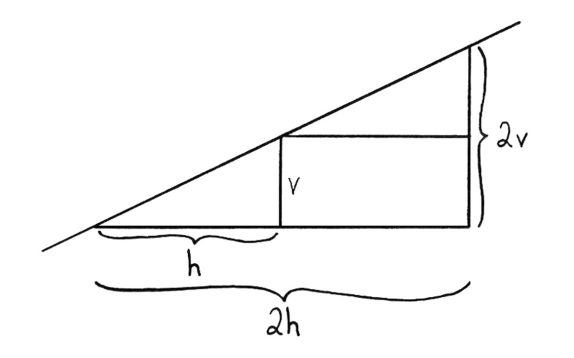
\includegraphics[width=10cm]{images/burn_math_1-8.png}
  \label{fig:1-8}
  \caption{captionだよ}
\end{figure}

\subsection{直線を表現してみよう}

直線がある装置$M(x)$で表されているとする。どんな数$x, \tilde{x}$に対しても、以下がなりたつはず

\[ \frac{(1点の垂直位置) - (もう1点の垂直位置)}{(1点の水平位置) - (もう1点の水平位置)} \equiv \frac{垂直距離}{水平距離} \equiv \frac{M(x) - M(\tilde{x})}{x - \tilde{x}}  = \# \]

つまりどの2点間をえらんでも、傾きは一定(\#)となる。 そして、(たまたま) $\tilde{x}$が0の場合

\begin{align*}
  \frac{M(x) - M(0)}{x} = \# \\
  M(x) = \#x + M(0)
\end{align*}

M(0)は一部でy切片とよばれ、\#とM(0)を別の略号に書き直すと

\[ M(x) = ax + b \]

となり、おなじみの直線の文になった。

\subsection{近道の公式}

\begin{figure}[h]
  \centering
  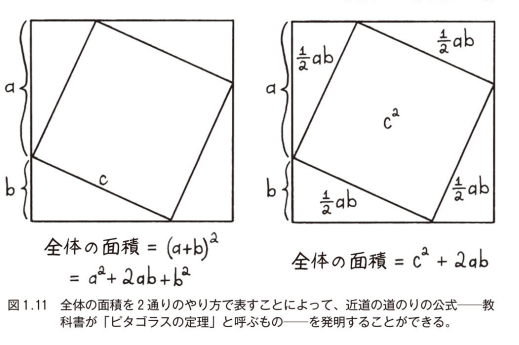
\includegraphics[width=10cm]{images/burn_math_1-11.png}
\end{figure}

\begin{align*}
  c^2 + 2ab &= a^2 + 2ab + b^2 \\
  c^2 &= a^2 + b^2
\end{align*}

\subsection{三角関数}

\subsubsection{装置の意味}

\begin{figure}[h]
  \centering
  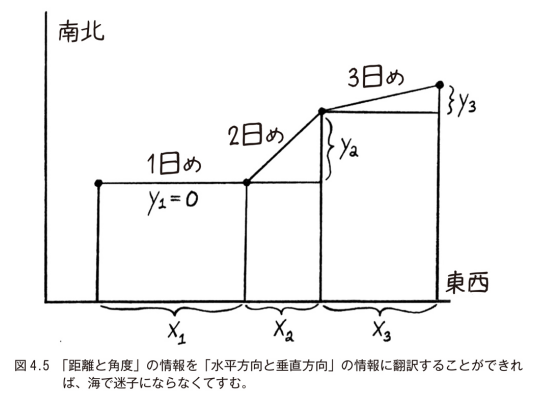
\includegraphics[width=10cm]{images/burn_math_4-5.png}
\end{figure}

いま航海をおこなっているとする、日々えられる情報はどの方角にどの程度進んだか。この情報から、水平方向にどのくらい、垂直方向にどのくらいかを抽出できれば、迷子にならない。

\begin{figure}[h]
  \centering
  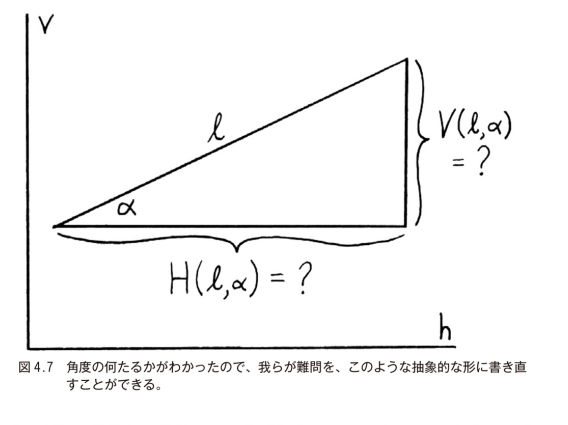
\includegraphics[width=10cm]{images/burn_math_4-7.png}
\end{figure}

問題をもうすこし抽象化すると、直線lと水平軸から反時計まわりの角度aが与えられた時、水平方向と垂直方向の長さをえる方法があるかということになる。垂直方向をV(l,a), 水平方向をH(l,a)で出力する装置を考える。

\begin{figure}[h]
  \centering
  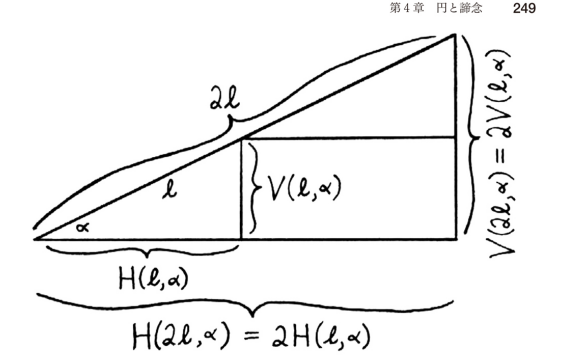
\includegraphics[width=10cm]{images/burn_math_4-8.png}
\end{figure}

直線をn倍すると垂直、水平方向もn倍されるので以下が成り立つ。

\[ H(nl,a) = nH(l,a) \]
\[ V(nl,a) = nV(l,a) \]

そうするといつものように、$l= l \cdot 1$ とみなして以下が成り立つ

\[ H(l\cdot 1,a) = lH(1,a) \]
\[ V(l\cdot 1,a) = lV(1,a) \]

すなわち、ある特定の(この場合1)の値さえ求められれば、その値をl倍することで、どんな直線にも対応できることになる。ということで、1を省略して以下のようにかけ、これがいわゆる$\sin, \cos$になる。

\[ H(1,a) \equiv H(a) \equiv \cos a \]
\[ V(1,a) \equiv V(a) \equiv \sin a \]

\subsubsection{装置を記述してみよう}

多項式は一般にいかのようにかける。

\[ M(x) = C_0x^0 + C_1x^1 + C_2x^2 + C_3x^3 + \cdots \]

これを微分して、0を代入すると

\[ M'(x) = 0 + (1)C_1 + (2)C_2x^1 + (3)C_3x^2 + \cdots \]
\[ M'(0) = C_1 \]

一般化すると、n回微分して0を代入することで、$C_nx^n$の左側はすべて消え、右側はxをひとつ含んでいて、0が代入されるので

\begin{align*}
M^{(n)}(0) &= C_nn! \\
C_n &= \frac{M^{(n)}(0)}{n!}
\end{align*}

したがって、多項式は以下のようにあらわせる

\begin{align*}
M(x) &= M(0) + \biggl( \frac{M^{(1)}(0)}{1!}\biggl)x + \biggl( \frac{M^{(2)}(0)}{2!}\biggl)x^2 + \biggl( \frac{M^{(3)}(0)}{3!}\biggl)x^3 + \cdots \\
M(x) &= \sum_{n=0}^{\infty}\frac{M^{(n)}(0)}{n!}x^n
\end{align*}

ということは、$\sin x$なるV(x)も以下のように記述できる

\[ V(x) = \sum_{n=0}^{\infty} \frac{V^{(n)}(0)}{n!}x^n \]

V(x)の微分は循環するので、以下のようにあらわせる

\begin{align*}
V^{(0)}(0) &= V(0) = 0 \\
V^{(1)}(0) &= H(0) = 1 \\
V^{(2)}(0) &= H'(0) = -V(0) = 0 \\
V^{(3)}(0) &= (-V)'(0) = -(V)'(0) = -H(0) = -1 \\
V^{(4)}(0) &= (-H)'(0) = -(H)'(0) = V(0) = 0
\end{align*}

偶数回の微分は0で奇数回は1と-1を繰り返すので、以下のようにかける。

\[ V(x) = x - \frac{x^3}{3!} + \frac{x^5}{5!} - \frac{x^7}{7!} + \cdots \]

同様にH(x)はこうかける。

\begin{align*}
H^{(0)}(0) &= H(0) = 1 \\
H^{(1)}(0) &= -V(0) = 0 \\
H^{(2)}(0) &= (-V)'(0) = -(V)'(0) = -H(0) = -1 \\
H^{(3)}(0) &= (-H)'(0) = -(H)'(0) = V(0) = 0 \\
H^{(4)}(0) &= V'(0) = H(0) = 1 \\
\\
H(x) = 1 - \frac{x^2}{2!} + \frac{x^4}{4!} - \frac{x^6}{6!} + \cdots
\end{align*}

\begin{figure}[h]
  \centering
  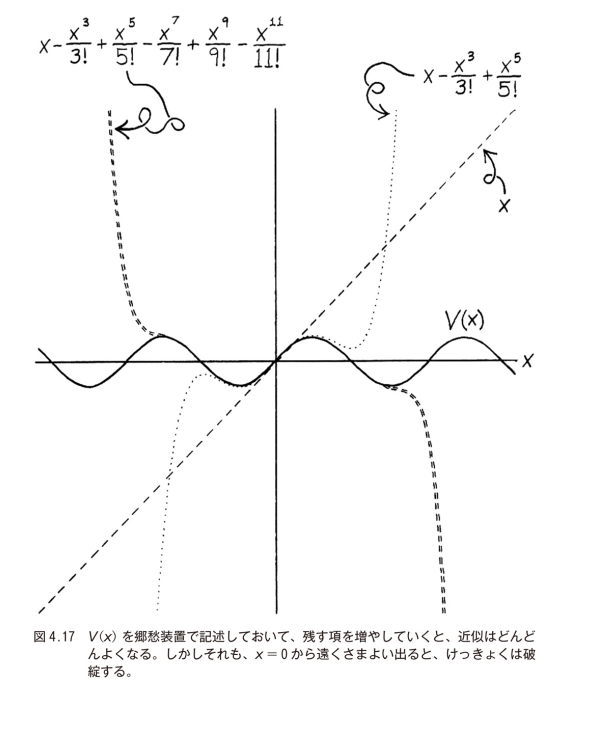
\includegraphics[width=10cm]{images/burn_math_4-17.png}
\end{figure}

\subsection{指数}

$(c)^n \equiv \underbrace{c \cdot c \cdots c}_{n回}$のように指数をその数をn回かけると定義してしまうと、nがマイナスだったり、分数の場合にマイナス1回かけるや、1/2回かけるとなって、うまく定義できない。 そこで、指数を以下のように定義する

\[(c)^{n+m} = (c)^n(c)^m \]

このように定義すると$C^0 = 1$が導かれる。

\[ (c)^n = (c)^{n+0} = (c)^n(c)^0 \]

また、負のべき乗は以下のようになる

\begin{align*}
1 &= (c)^0 = (c)^{n-n} = (c)^{n+(-n)} = (c)^n(c)^{-n} \\
(c)^{-n} &= \frac{1}{(c)^n}
\end{align*}

分数のべき乗は、自身をn回かけると元の数になるものになる

\[ c = (c)^1 = (c)^{\frac{n}{n}} = (c)^{\sum_{i=1}^{n}\frac{1}{n}} = \prod_{i=1}^{n}(c)^{\frac{1}{n}} \]

\section{微分}

\subsection{定義}
まがったグラフの傾きをどのように表現するか。まがっているものは扱えないので、ある1点を無限に拡大してそこに直線をみいだすというアプローチを採用する。そうすると点xでの傾きは

\[ xにおけるMの傾向 \equiv \frac{極小垂直変位}{極小水平変位} \equiv \frac{垂直距離}{水平距離} \equiv \frac{M(x+極小) - M(x)}{(x + 極小) -x } \]

  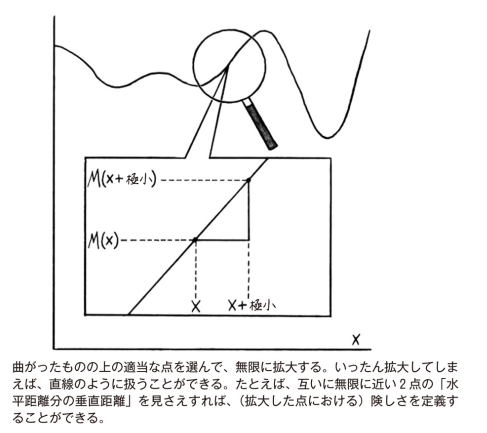
\includegraphics[width=10cm]{images/burn_math_2-1.png}

\subsubsection{水平線で試してみる}

$M(x) \equiv 7$というなにをいれても7を出力する装置で微分を試してみる。

\[ xにおけるMの傾き \equiv \frac{M(x + 極小) - M(x)}{極小} = \frac{7-7}{極小} = 0(\frac{1}{極小}) = 0 \]

上の文では、7という数固有の性質に一切依拠していないので、$M(x) = \#$ という形の装置はすべてのxにおいて傾きが0となる


\subsubsection{直線で試してみる}

直線はM(x) = ax + bという形の装置であることはわかっているので、微分してみると

\[ xにおけるMの傾き \equiv \frac{M(x + 極小) - M(x)}{極小} = \frac{[a \cdot (x + 極小) + b] - [ax + b]}{極小} = \frac{a \cdot (極小)}{極小} = a \]

となり、直線の傾きは常に一定であるという事実と符合する結果となる!

\subsubsection{本当に曲がっているもので試してみる}

$M(x) = x^2$という装置で試してみる。

\begin{align*}
  xにおけるMの傾き &\equiv \frac{M(x + 極小) - M(x)}{極小} = \frac{(x + 極小)^2 - x^2}{極小} \\
  &= \frac{x^2 + 2x(極小) + (極小)^2 - x^2}{極小} \\
  &= \frac{2x(極小) + (極小)^2}{極小} \\
  &= 2x + 極小
\end{align*}

2x + 極小は, 2xに無限に近いので、2xと扱っても矛盾はおきないと考えると、$M(x) = x^2$におけるxの傾きは2xとなる。

\subsubsection{極限を整理しよう}

うえの文は、$lim$ という記号を使って以下のようにも表せる

\begin{align*}
  M'(x) &\equiv \lim_{h \to 0} \biggl[ \frac{M(x+h)-M(x)}{h}\biggr] = \lim_{h \to 0} \biggl[ \frac{(x+h)^2 -x^2}{h}\biggr] = \lim_{h \to 0} \biggl[ \frac{(2xh + h^2)}{h}\biggr] \\
  &= \lim_{h \to 0}[2x +h] = 2x
\end{align*}

まずこのダッシュは、「M(x)を拡大し、それが直線であるかのように考えて傾きをもとめる」ことを意味する略号で、Mプライムxと読む。

$lim$という記号については、わたしの内側のすべてをhがごく日常的な数であって、無限に小さな数でないふりをして計算せよ。そして下半分にあるhをすべて追い払うことができたら(ゼロで割る心配をしなくてよくなったら),hのつまみをぐいっとまわして、hがどんどんちいさくなるところを想像する。

\subsubsection{略号を整理しよう}

以下の略号はすべておなじ概念をいわんとしている。それぞれ強調している点があるので、コンテキストで使い分けると議論がしやすい。
\begin{enumerate}
 \item xにおけるMの傾き

 \item xにおけるMの微分係数(differential coefficient)

微分係数というのは名詞で、動詞「微分する」は「微分係数を求める」を意味する

 \item $M'(x)$

 これは傾きを吐き出す装置を考えることができるという事実を強調した略号。$M'(x)$はそこにxをいれるとその点xにおける元の装置Mの傾きを吐き出す装置を表す。いわゆる導関数

 \item $\frac{dM}{dx}$

 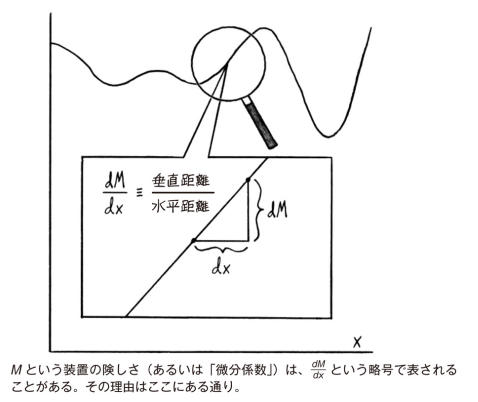
\includegraphics[width=10cm]{images/burn_math_2-2.png}

 装置Mの微分係数や導関数がこう書かれることがある

\subsection{$x^n$の微分}
\begin{align*}
M(x) &= x^n とすると \\
M'(x) &= \frac{M(x+t)-M(x)}{t} = \frac{(x+t)^n - x^n}{t} \\
&= \frac{x^n - x^n + \binom {n}{1}x^{n-1}t^1 + t^2(...)}{t} \qquad \text{(二項定理から)} \\
&=  \binom{n}{1} x^{n-1} \qquad \text{($\frac{1}{t}をかけたあとにもtが残っている項はすべて0になる$)} \\
&= nx^{n-1}
\end{align*}

\subsection{定数倍の微分}

$m(x) \equiv cf(x)$ (cは定数)のように、mは装置fの定数倍を出力するものとすると
\[ m'(x) = \frac{m(x+t) - m(x)}{t} = \frac{cf(x+t) - cf(x)}{t} = c \biggl( \frac{f(x+t) -f(x)}{t} \biggl) = cf'(x) \]

このことは以下のように表現できる
\begin{align*}
  m(x) &\equiv cf(x) \rightarrow m'(x) \equiv cf'(x) \\
  [cf(x)]' &= cf'(x) \\
  \frac{\mathrm{d}}{\mathrm{d}x}[cf(x)] &= c\frac{\mathrm{d}}{\mathrm{d}x}f(x) \\
  (cf)' &= c(f')
\end{align*}

\subsection{和の微分}

$M(x) \equiv f(x) + g(x)$という装置を考えてみる。これは実際には2つの小さな装置f,gの出力をあわせた装置をひとつの装置としてみているともいえる。

\begin{align*}
M'(x) &= \frac{M(x+t)-M(x)}{t} = \frac{[f(x+t)+g(x+t)] - [f(x)+g(x)]}{t} \\
&= \frac{f(x+t)-f(x) + g(x+t) -g(x)}{t} \\
&= \frac{f(x+t)-f(x)}{t} + \frac{g(x+t) -g(x)}{t} \\
&= f'(x) + g'(x)
\end{align*}

これは、ある装置を別の2つ装置の和とみなすと、その装置の微分は、小さな2つの装置の微分の和で求めることができることを示している。まだ2つの場合だけしかいえないので、n個に拡張したい。n=2の場合はわかったので、数学的帰納法でkならばk+1を示す。

\begin{align*}
&(f_1+f_2+...+f_k)' = f_1' + f_2' + ... + f_k' がなりたつと仮定すると \\
&(f_{k+1} + (f_1 + f_2 + ... + f_k))' = f_{k+1}' + (f_1 + f_2+ ... + f_k)' \\
&f_1' + f_2' + ... + f_k' + f_{k+1}' がいえる。
\end{align*}

したがって以下のように、いわゆる和の微分は、微分の和がいえる。
\begin{align*}
  M(x) & \equiv \sum_{i=1}^{n}f_{i}(x) \equiv f_1(x) + f_2(x) + ... + f_{n}(x) とすると \\
  M'(x) & \equiv \Bigl[ \sum_{i=1}^{n}f_{i}(x) \Bigl]' = \sum_{i=1}^{n}[f_{i}(x)]'
\end{align*}

\subsection{多項式の微分}

$x^n$、定数倍、和でつながった複数の関数の微分がそれぞれ定義できたので、いよいよ多項式の微分ができる!

\begin{align*}
 M(x)' &= \biggl[ \sum_{k=0}^{n}C_kx^k \biggl]' &\equiv \biggl[ C_0x^0 + C_1x^1 + ... + C_nx^n \biggl]' \\
 &= \sum_{k=0}^{n}\biggl [C_kx^k \biggl]' &\equiv [C_0x^0]' + [C_1x^1]' + ... + [C_nx^n]' \\
 &= \sum_{k=0}^{n}C_k \biggl[x^k\biggl]' &\equiv C_0[x^0]' + C_1[x^1]' + ... + C_n[x^n]' \\
 &= \sum_{k=0}^{n}C_k kx^{k-1}
\end{align*}

\subsection{積の微分}

\begin{align*}
M(x) &\equiv f(x)g(x) \\
M(x)' &= \frac{f(x+t)g(x+t)-f(x)g(x)}{t} \\
&= \frac{f(x+t)g(x+t)-f(x)g(x) + \overbrace{f(x)g(x+t)-f(x)g(x+t)}^{ウソと訂正}}{t} \\
&= \frac{f(x)g(x+t)-f(x)g(x) + f(x+t)g(x+t)-f(x)g(x+t)}{t} \\
&= f(x)\biggl( \frac{g(x+t)-g(x)}{t} \biggl) + \biggl( \frac{f(x+t)-f(x)}{t}\biggl)g(x+t) \\
&= f(x)g'(x) + f'(x)g(x) \\
したがって、(fg)' &= f'g + g'f
\end{align*}

\subsection{三角関数の微分}

\begin{figure}[h]
  \centering
  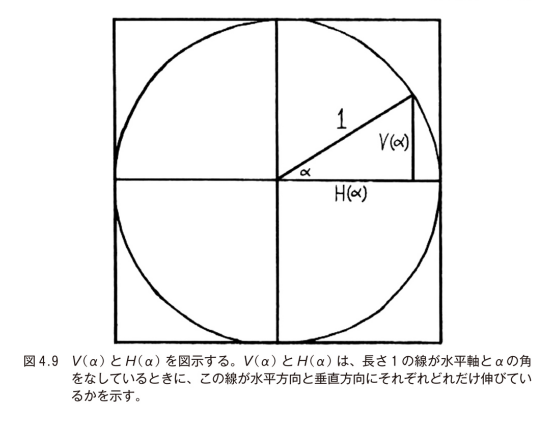
\includegraphics[width=10cm]{images/burn_math_4-9.png}
\end{figure}

三角関数の微分は、角度aをわずかに増やしたとき、V(a)はどのように変化するかを考えること。

\begin{figure}[h]
  \centering
  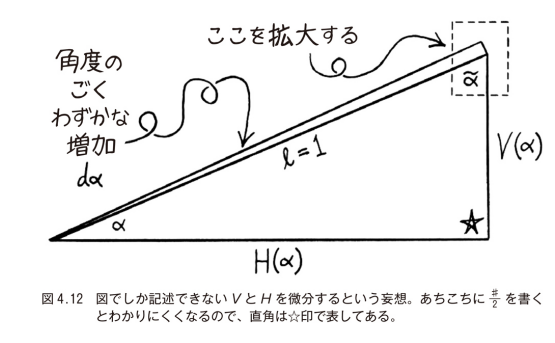
\includegraphics[width=10cm]{images/burn_math_4-12.png}
\end{figure}


角度aを無限に小さい量daだけ増やした時、4-13の図の左にのびる2本の直線は平行になっているはず。(あるいは無限に平行に近い)これは直感に反するが、もし、この2本が平行でないとすると、この2本に間には測定可能なゼロより確実に大きい、角度があることになり、daが無限に小さいことにならなくなる。(奇妙な推論)

下の図から、$☆ + \tilde{a} + ? = \pi $、そして元の三角形は$☆+ \tilde{a} + a = \pi$ なので、代入すると$? = a$がなりたち、元の三角形と拡大したことによってできた三角形は相似であることがわかる。

\begin{figure}[h]
  \centering
  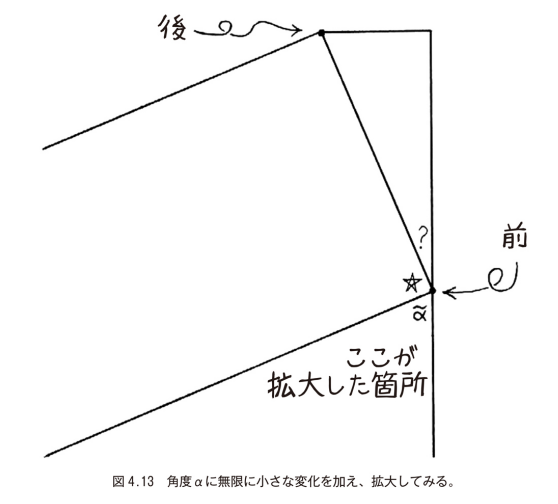
\includegraphics[width=10cm]{images/burn_math_4-13.png}
\end{figure}

\begin{figure}[h]
  \centering
  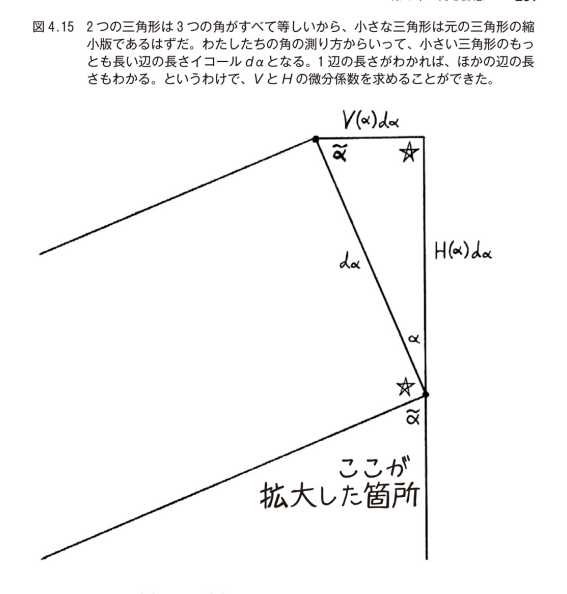
\includegraphics[width=10cm]{images/burn_math_4-15.png}
\end{figure}


角度の図り方から、全円は$2\pi$となる。ところが、$2\pi$は半径1の円の円周の長さでもあって、半径1の円では、角度がそのまま、道のりになる。したがって、ふたつの$\tilde{a}$を結ぶ線の長さは半径が描いた角度そのものだから、daになる。

この図から

\begin{align*}
dV &= H(a)da \\
\frac{dV}{da} &= H(a) \\
\\
dH &= -V(a)da \\
\frac{dH}{da} &= -V(a)
\end{align*}

教科書てきには

\begin{align*}
  \frac{d}{dx}\sin (x) &= \cos (x) \\
  \frac{d}{dx}\cos (x) &= -\sin (x)
\end{align*}


\end{enumerate}
\end{document}